\begin{frame}
    \frametitle{Научная новизна}
    \begin{enumerate}
        \item Установлено естественное соответствие между булевыми правильными семействами и одностоковыми ориентациями графов булевых кубов ($\uso$-ориентации), а также между булевыми правильными семействами и булевыми сетями с наследственно единственной неподвижной точкой ($\hupf$-сети); установлено естественное соответствие между правильными семействами в логике произвольной значности и кликами в обобщенных графах Келлера.
        \item Доказано, что стабилизатором множества правильных семейств функций являются изометрии пространства Хэмминга (согласованные перенумерации и перекодировки); 
        \item Показано, что отображения, задаваемые с помощью правильных семейств булевых функций, всегда имеют четное число неподвижных точек.
        \item Получена оценка на число правильных семейств булевых функций, предложены оценки доли треугольных семейств среди всех правильных семейств булевых функций.
    \end{enumerate}
\end{frame}


\begin{frame}
    \frametitle{Научная новизна}
    \begin{enumerate}
        \item Обнаружены и исследованы новые классы правильных семейств функций (рекурсивно треугольные, локально треугольные, сильно квадратичное семейство); получены оценки на число рекурсивно треугольных семейств; для некоторых правильных семейств булевых функций получены точные значения мощности образа отображений, задаваемых этими правильными семействами.
        \item Предложен новый способ порождения квазигрупп на основе правильных семейств функций; доказан ряд утверждений о числе ассоциативных троек в порождаемых квазигруппах.
        \item Предложен новый алгоритм шифрования, сохраняющего формат ($\fpe$-схема), основанный на квазигрупповых операциях.
    \end{enumerate}
\end{frame}


\begin{frame}
    \frametitle{Отзыв на НКР-1}
    \centering
    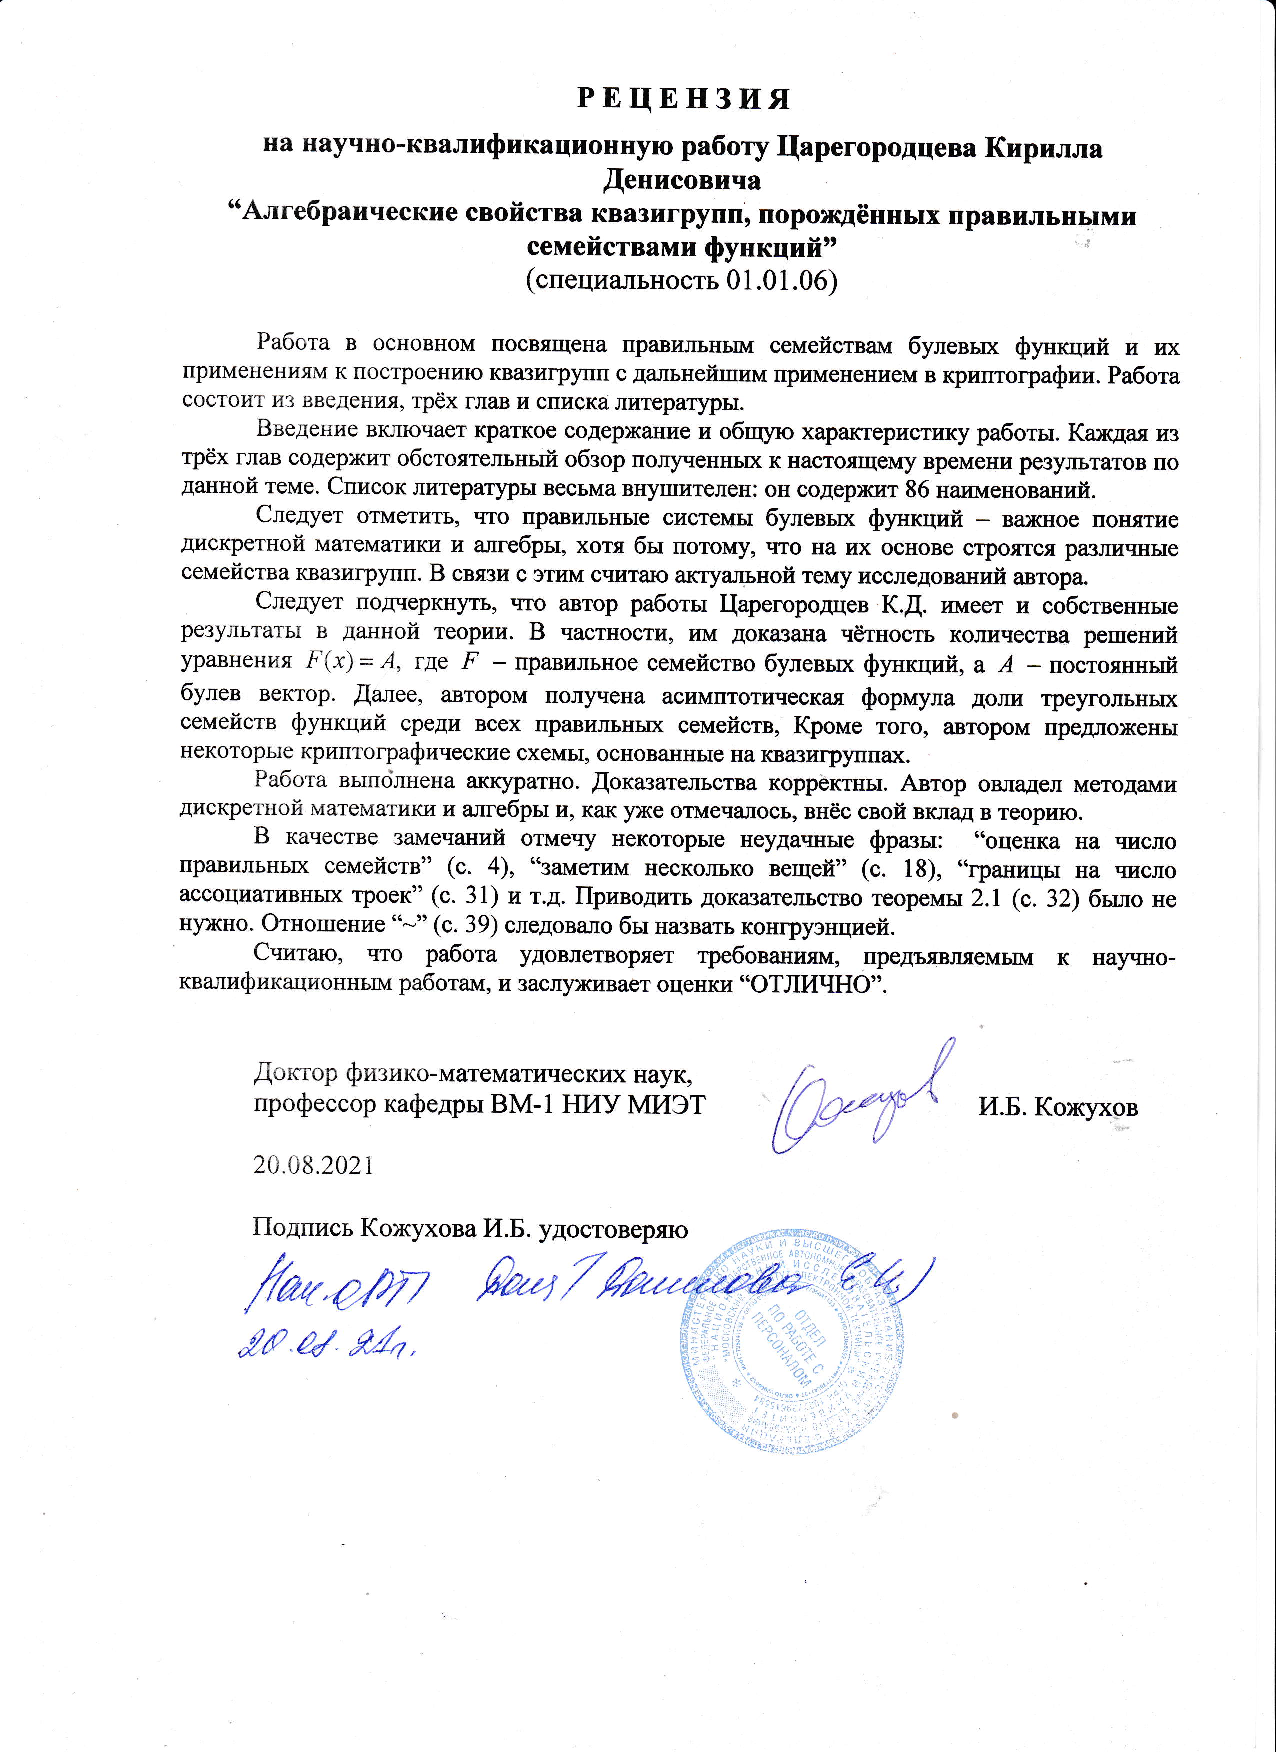
\includegraphics[width=0.7\linewidth]{review_outer}
\end{frame}

\begin{frame}
    \frametitle{Отзыв на НКР-2}
    \centering
    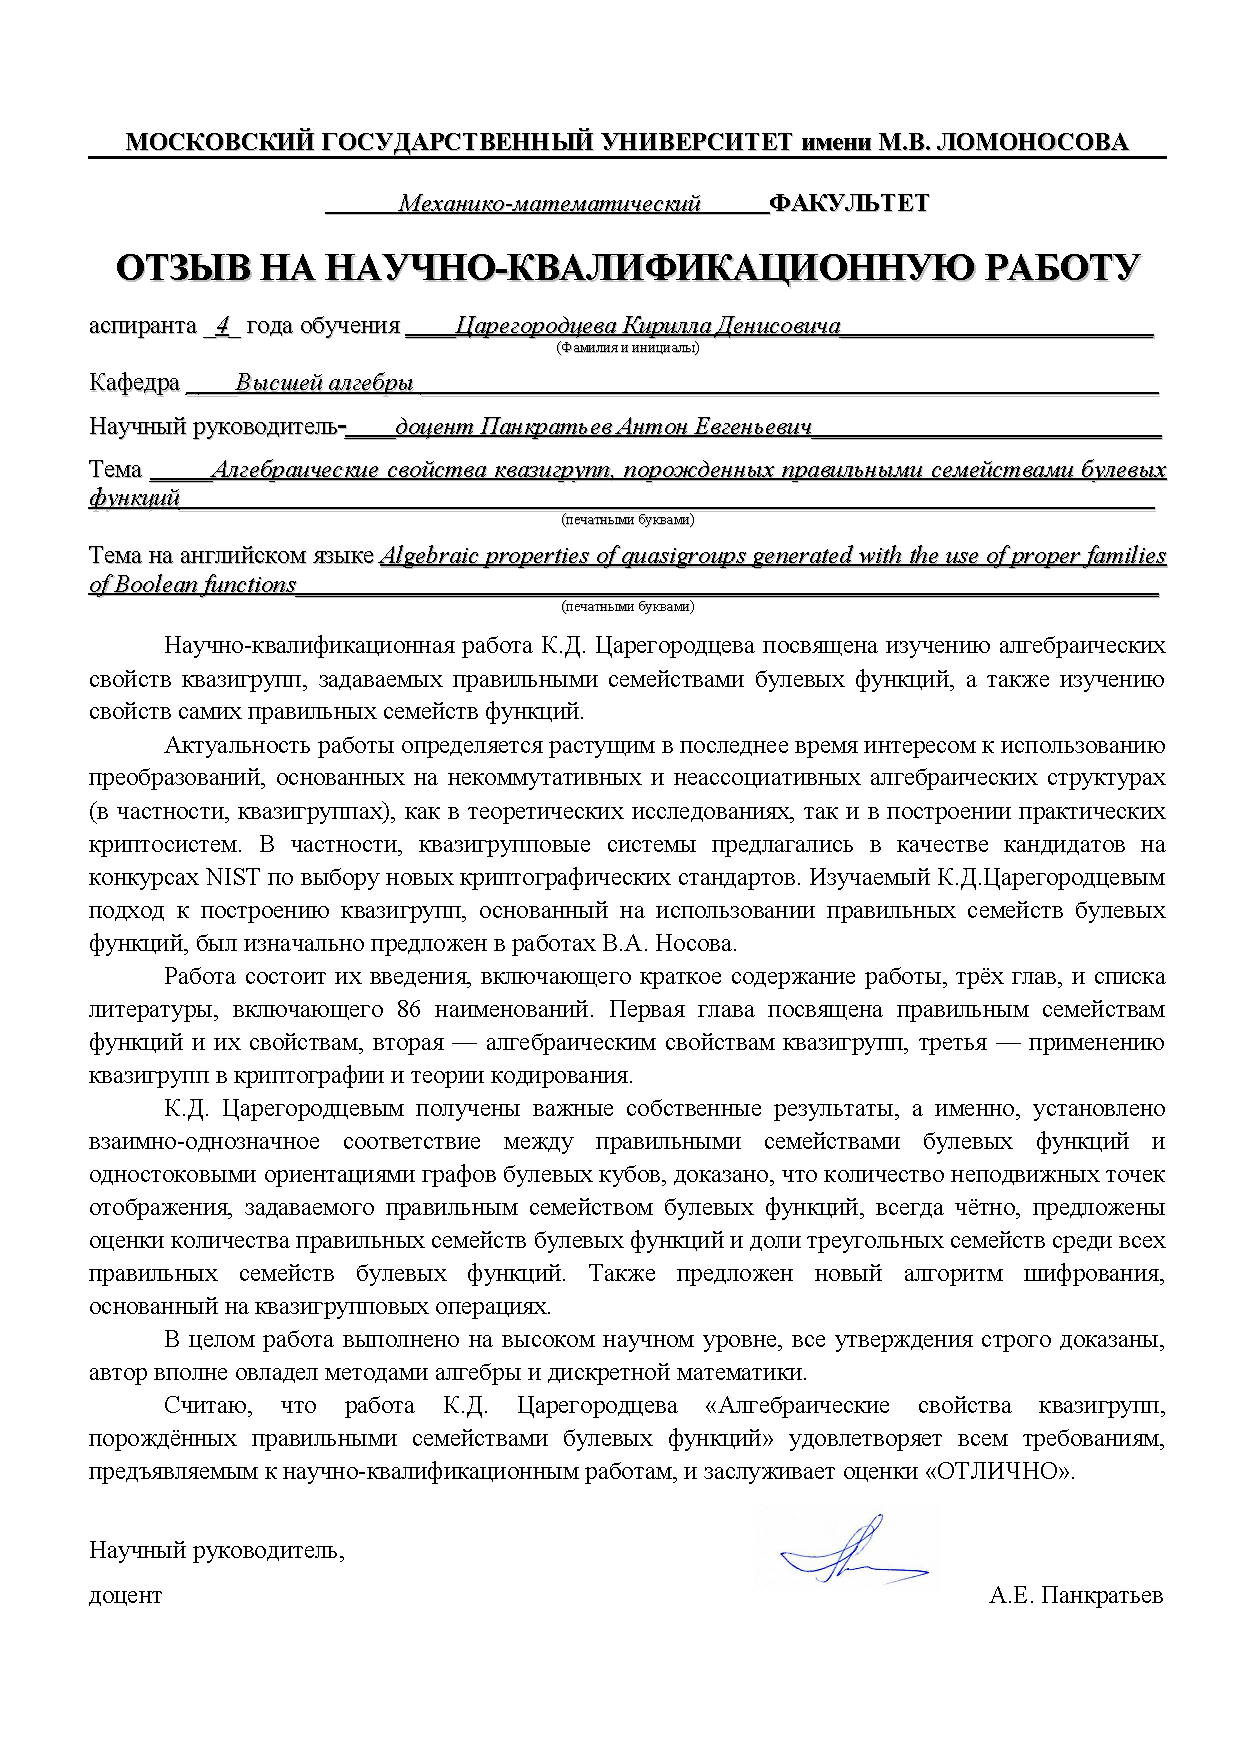
\includegraphics[width=0.6\linewidth]{review_inner}
\end{frame}

\begin{frame}
    \frametitle{Заключение кафедры}
    \centering
    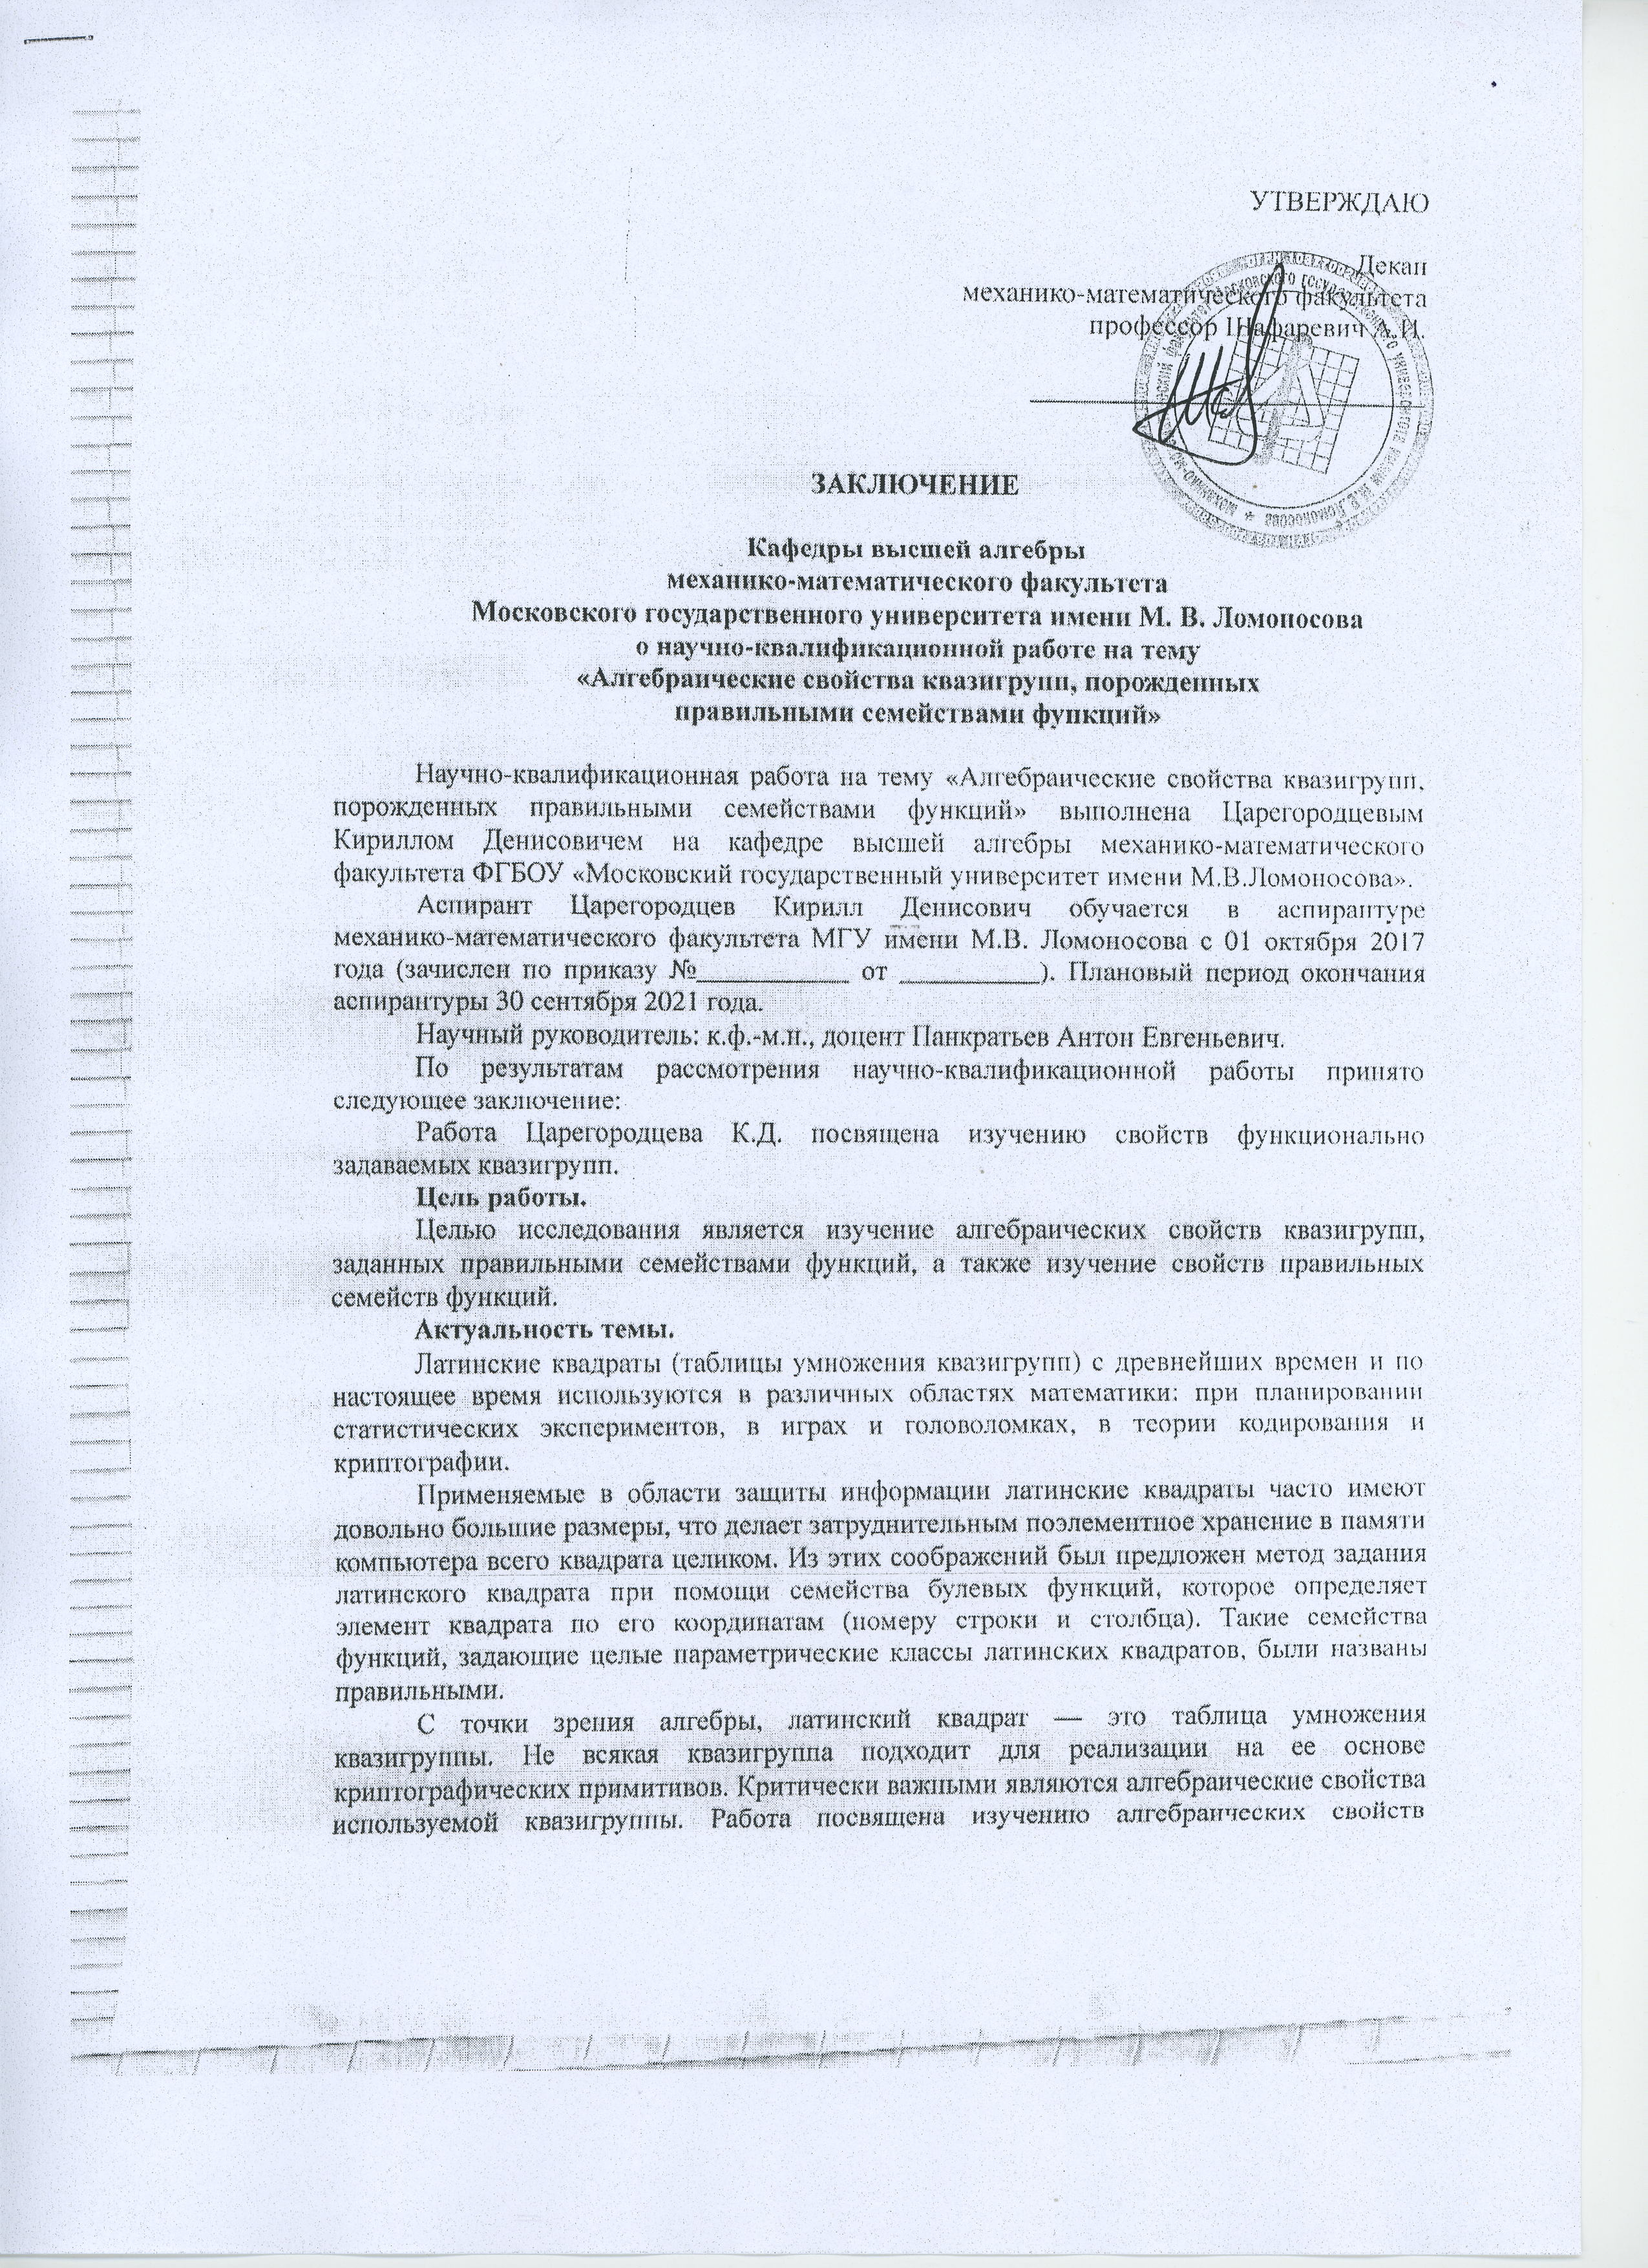
\includegraphics[width=0.65\linewidth]{kaf1}
\end{frame}

\begin{frame}
    \frametitle{Заключение кафедры}
    \centering
    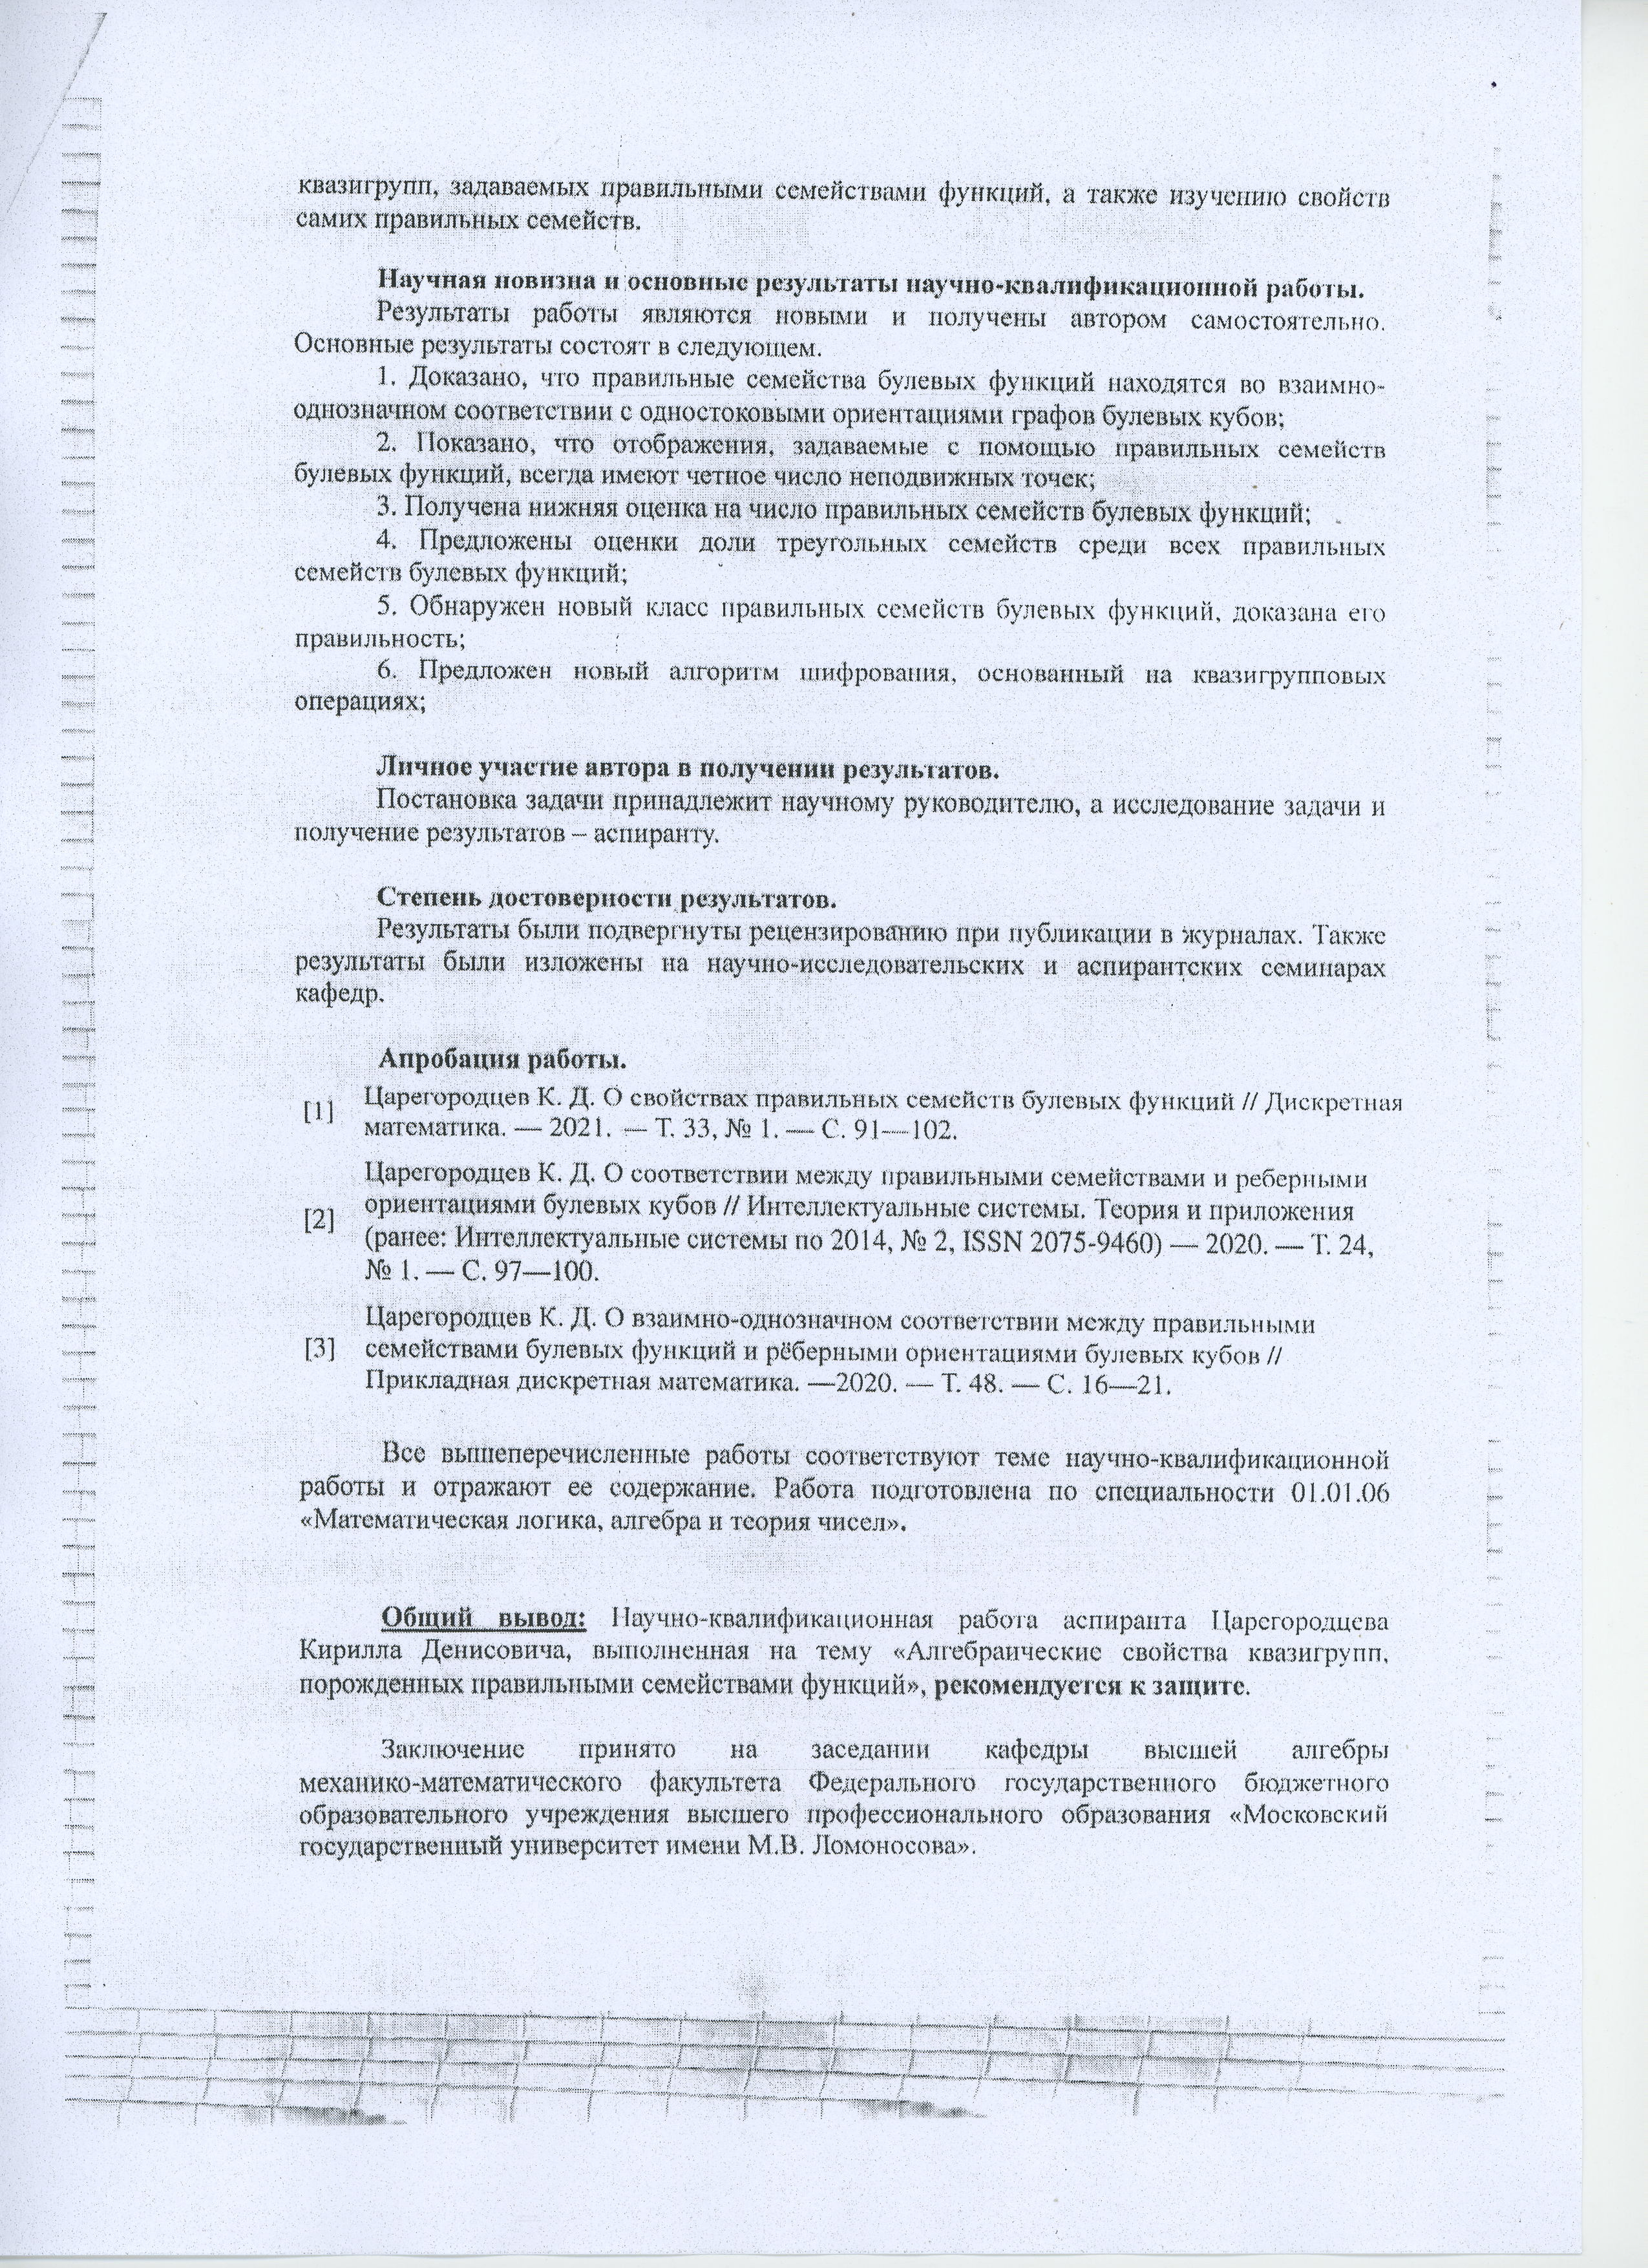
\includegraphics[width=0.65\linewidth]{kaf2}
\end{frame}

\begin{frame}
    \frametitle{Заключение кафедры}
    \centering
    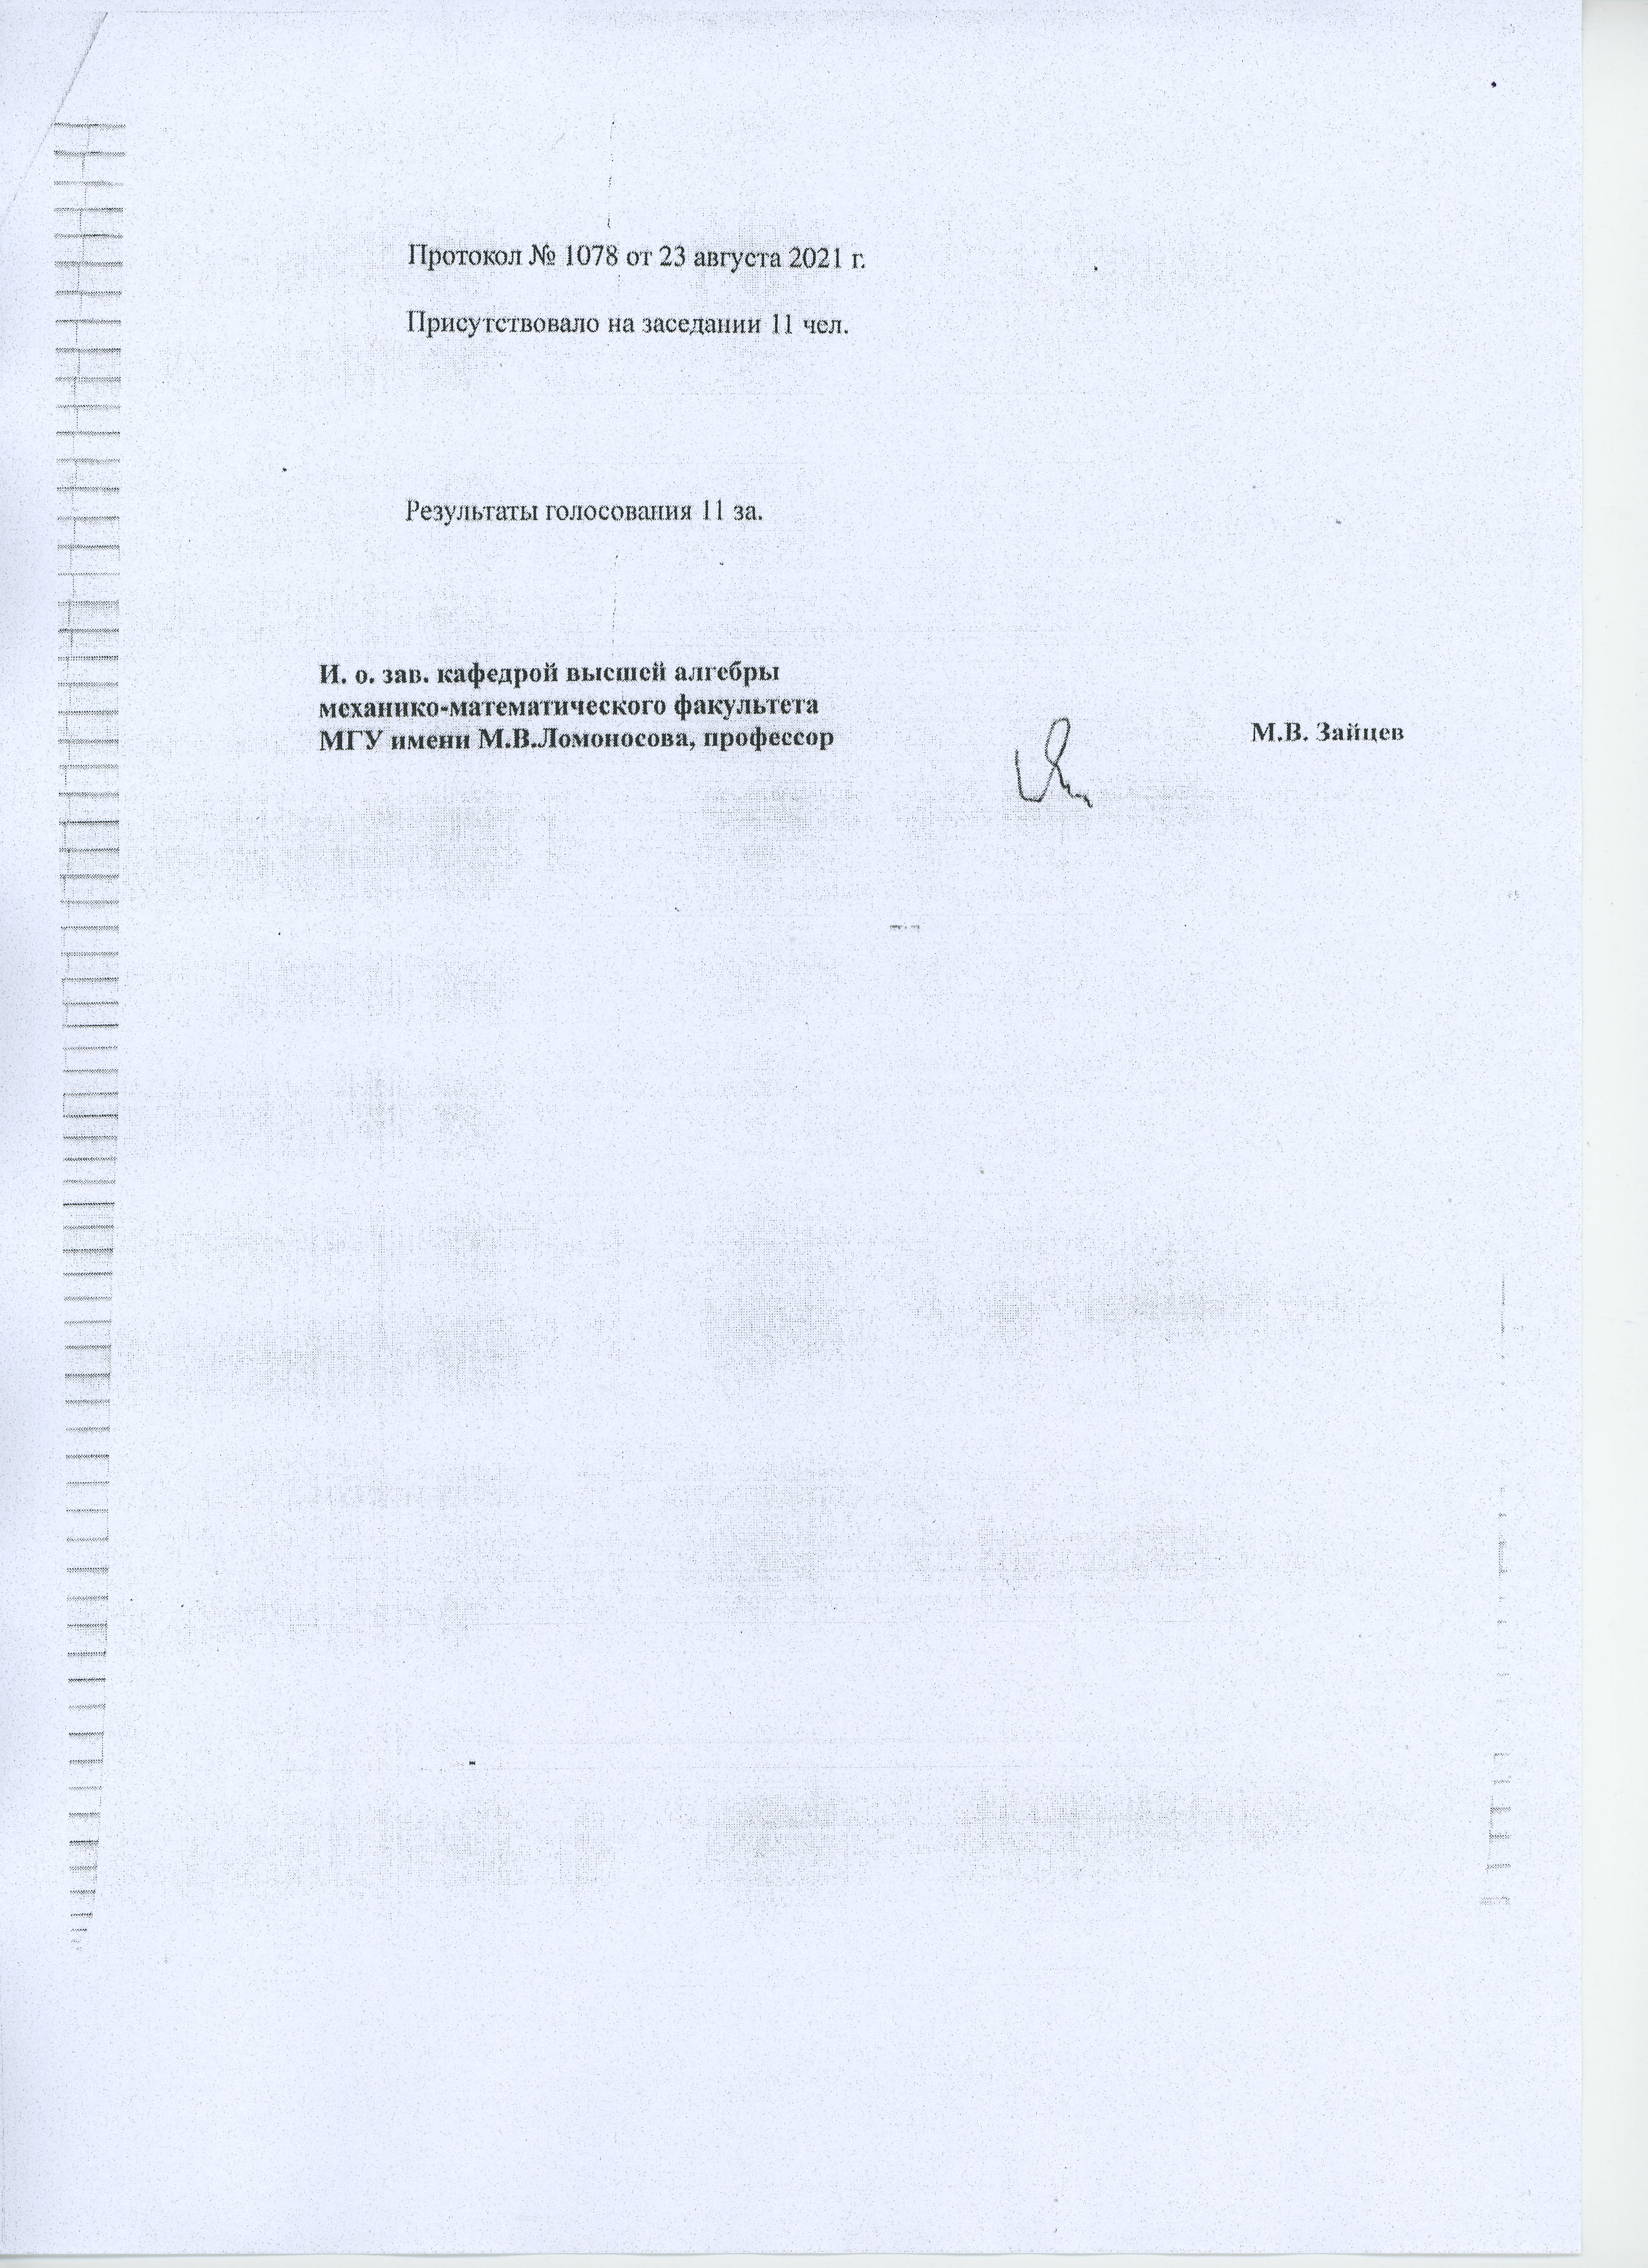
\includegraphics[width=0.75\linewidth]{kaf3}
\end{frame}

\begin{frame} % публикации на одной странице
% \begin{frame}[t,allowframebreaks] % публикации на нескольких страницах
    \frametitle{Основные публикации}
    \nocite{intsys20}
    \nocite{pdm20}
    \nocite{dm21}
    \nocite{fpe22}
    \nocite{galatenko23}
    \nocite{galatenko2023proper}
    \nocite{fpm23}
    \nocite{sibecrypt23}
    \nocite{tsar24}
    \ifnumequal{\value{bibliosel}}{0}{
        \insertbiblioauthor
    }{
        \printbibliography%
    }
\end{frame}

\begin{frame}
\frametitle{Участие в конференциях}
    \begin{itemize}
        \item XXVI Международная конференция студентов, аспирантов и молодых учёных <<Ломоносов>>, Москва, Россия, 2019~г.;
    
        \item X симпозиум <<Современные тенденции в криптографии>> (CTCrypt 2021), Дорохово, Россия, 2021~г.;
    
        \item XI симпозиум <<Современные тенденции в криптографии>> (CTCrypt 2022), Новосибирск, Россия, 2022~г.;
        
        \item 11-я Международная конференция <<Дискретные модели в теории управляющих систем>>, Красновидово, Россия, 2023~г.;
    \end{itemize}
\end{frame}

\begin{frame}{Участие в конференциях}
    \begin{itemize}
        \item Третья Международная конференция ``MATHEMATICS IN ARMENIA: ADVANCES AND PERSPECTIVES'', Ереван, Армения, 2023~г.;
    
        \item 22-я Международная конференция <<Сибирская научная школа-семинар ``Компьютерная безопасность и криптография'' имени Геннадия Петровича Агибалова>>, Барнаул, Россия, 2023~г.;
    
        \item Международная конференция <<Математика в созвездии наук>>, Москва, Россия, 2024~г.;
    
        \item Международная конференция <<Алгебра и математическая логика: теория и приложения>>, Казань, Россия, 2024~г.;
    
        \item XX Международная научная конференция <<Проблемы теоретической кибернетики>>, Москва, Россия, 2024~г.
    \end{itemize}
\end{frame}

\begin{frame}[plain, noframenumbering] % последний слайд без оформления
    \begin{center}
        \Huge
        Спасибо за внимание!
    \end{center}
\end{frame}
